% Standalone source to regenerate fig/04_events/selection_flow_bdt.pdf
% BDT-preselection variant of selection_flow.tex (fig:selectionflow), kept in the
% same layout. Differences w.r.t. the cut-based flow, from
% Analyzers/src/HNWR_BDT_presel_3SR.cc of SKNanoAnalyzer-v13:
%   * mass cuts dropped   : mll>400, mlljj>800, mlJ>800  -> BDT inputs
%   * AK8 cuts dropped    : LSF3>0.75, SDM>40, |dphi(l,J)|>2.0 -> BDT inputs
%   * lead lepton pT      : 130 (e) / 60 (mu) instead of 60
%   * third signal region : boosted_nolep, for boosted events with no extra
%                           loose lepton at all (N-side lepton unreconstructed)
% Build (from repo root):
%   fig/04_events/scripts/build_selection_flow_bdt.sh
% or, where standalone.cls is installed:
%   cd fig/04_events && lualatex -interaction=nonstopmode selection_flow_bdt.tex

% standalone.cls is not present on every machine; fall back to a big-page
% article that is cropped afterwards by the build script.
\IfFileExists{standalone.cls}
  {\documentclass[border=2pt]{standalone}}
  {\documentclass{article}%
   \usepackage[margin=2pt,paperwidth=45cm,paperheight=45cm]{geometry}%
   \pagestyle{empty}}

\usepackage{tikz}
\usetikzlibrary{positioning,arrows.meta,calc}
\usepackage{xspace}

% Inside narrow text-width nodes TeX stretches \thickmuskip (5mu plus 5mu) rather
% than overfilling a line, which blows the spacing around < and > out to ~1em.
\thinmuskip=3mu
\medmuskip=4mu
\thickmuskip=5mu

\newcommand{\pt}{\ensuremath{p_{\mathrm{T}}}\xspace}
\newcommand{\mll}{\ensuremath{m_{\ell\ell}}\xspace}
\newcommand{\mlljj}{\ensuremath{m_{\ell\ell jj}}\xspace}
\newcommand{\mlJ}{\ensuremath{m_{\ell J}}\xspace}
\newcommand{\dR}{\ensuremath{\Delta R}\xspace}

\begin{document}

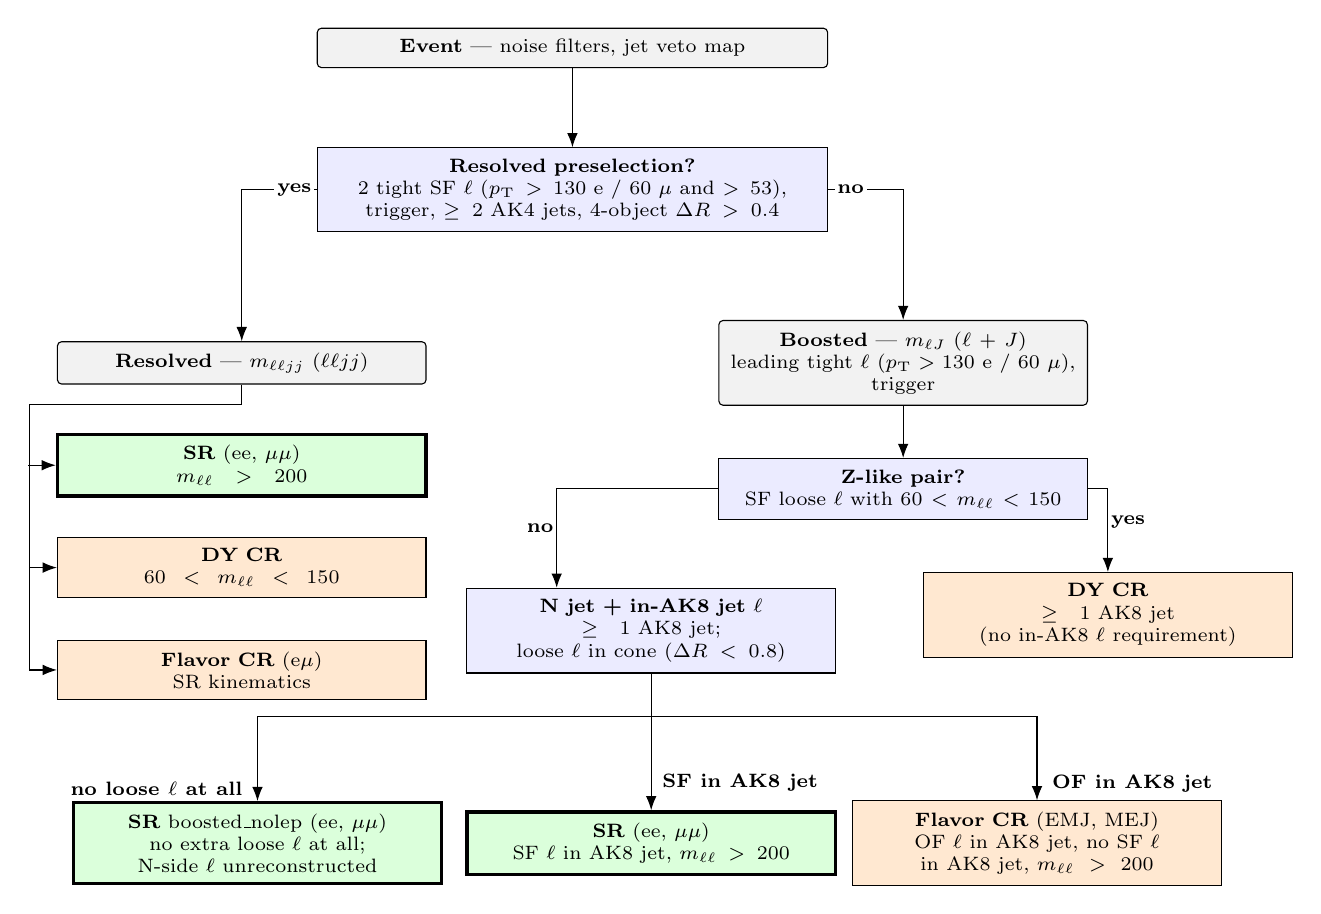
\begin{tikzpicture}[
    font=\scriptsize,
    box/.style={draw, rounded corners=1.5pt, align=center, inner sep=4pt, fill=gray!10, text width=44mm},
    dec/.style={draw, align=center, inner sep=4pt, fill=blue!8, text width=44mm},
    reg/.style={draw, very thick, align=center, inner sep=4pt, fill=green!14, text width=44mm},
    cr/.style={draw, align=center, inner sep=4pt, fill=orange!18, text width=44mm},
    lbl/.style={font=\scriptsize\bfseries, fill=white, inner sep=1pt, align=center},
    >={Latex[length=1.8mm]}]
  % top
  \node[box, text width=62mm] (evt) at (0.0, 0.0)
    {\textbf{Event} --- noise filters, jet veto map};
  \node[dec, text width=62mm] (res) at (0.0, -1.8)
    {\textbf{Resolved preselection?}\\ 2 tight SF $\ell$ ($\pt>130$ e / 60 $\mu$ and $>53$),\\
     trigger, $\geq 2$ AK4 jets, 4-object $\dR>0.4$};
  % ----- left column: resolved -----
  \node[box] (rhead) at (-4.2, -4.0) {\textbf{Resolved} --- $\mlljj$ ($\ell\ell jj$)};
  \node[reg] (rsr)  at (-4.2, -5.3) {\textbf{SR} (ee, $\mu\mu$)\\ $\mll>200$};
  \node[cr]  (rdy)  at (-4.2, -6.6) {\textbf{DY CR}\\ $60<\mll<150$};
  \node[cr]  (rflv) at (-4.2, -7.9) {\textbf{Flavor CR} (e$\mu$)\\ SR kinematics};
  % ----- right column: boosted -----
  \node[box] (bhead) at (4.2, -4.0) {\textbf{Boosted} --- $\mlJ$ ($\ell + J$)\\ leading tight $\ell$ ($\pt>130$ e / 60 $\mu$),\\ trigger};
  \node[dec] (bz)    at (4.2, -5.6) {\textbf{Z-like pair?}\\ SF loose $\ell$ with $60<\mll<150$};
  \node[cr]  (bdy)   at (6.8, -7.2) {\textbf{DY CR}\\ $\geq 1$ AK8 jet\\ (no in-AK8 $\ell$ requirement)};
  \node[dec] (bjet)  at (1.0, -7.4) {\textbf{N jet + in-AK8 jet $\ell$}\\ $\geq 1$ AK8 jet;\\
    loose $\ell$ in cone ($\dR<0.8$)};
  \node[reg] (bnolep) at (-4.0, -10.1) {\textbf{SR} boosted\_nolep (ee, $\mu\mu$)\\ no extra loose $\ell$ at all;\\ N-side $\ell$ unreconstructed};
  \node[reg] (bsr)   at (1.0, -10.1) {\textbf{SR} (ee, $\mu\mu$)\\ SF $\ell$ in AK8 jet, $\mll>200$};
  \node[cr]  (bflv)  at (5.9, -10.1) {\textbf{Flavor CR} (EMJ, MEJ)\\ OF $\ell$ in AK8 jet, no SF $\ell$ in AK8 jet, $\mll>200$};
  % ----- arrows -----
  \draw[->] (evt) -- (res);
  \draw[->] (res.west) -| node[lbl, pos=0.15]{yes} (rhead.north);
  \draw[->] (res.east) -| node[lbl, pos=0.15]{no}  (bhead.north);
  % parallel branches from the resolved header via a left-side bus
  \draw (rhead.south) -- ++(0,-0.25) -| ($(rhead.south west)+(-0.35,-0.25)$) coordinate (rbusstart);
  \draw (rbusstart) -- ($(rflv.west)+(-0.35,0)$);
  \foreach \leaf in {rsr,rdy,rflv}{
    \draw[->] ($(\leaf.west)+(-0.35,0)$) -- (\leaf.west);}
  \draw[->] (bhead) -- (bz);
  \draw[->] (bz.east)  -| node[lbl, pos=0.7, right]{yes} (bdy.north);
  \draw[->] (bz.west)  -| node[lbl, pos=0.7, left]{no}  ([xshift=-12mm]bjet.north);
  \draw[->] (bjet.south) -- ++(0,-0.55) -| node[lbl, pos=0.93, left, xshift=-1.5mm]{no loose $\ell$ at all} (bnolep.north);
  \draw[->] (bjet.south) -- ++(0,-0.55) -| node[lbl, pos=0.85, right, xshift=1mm]{SF in AK8 jet} (bsr.north);
  \draw[->] (bjet.south) -- ++(0,-0.55) -| node[lbl, pos=0.9, right, xshift=1.5mm]{OF in AK8 jet} (bflv.north);
\end{tikzpicture}

\end{document}
